\section{Experiments}
\label{sec:expt}

\subsection{Evaluation data}

\paragraph*{CoNLL:} 
The CoNLL dataset ~\cite{Hoffart2011} contains 1393 articles with
about 34K mentions, and the standard performance metric is
mention-averaged accuracy.  The documents are partitioned into train,
test-a and test-b. Like most authors, we report performance on the
231 test-b documents with 4483 linkable mentions.  


\paragraph*{TAC KBP:} 
The TAC KBP 2010, 2011, and 2012 evaluation datasets \cite{TAC2010,TAC2011,TAC2012} include 2250,
2250, and 2226 mentions (2012) respectively,
of which roughly half are linkable
to the reference KB.  The competition evaluation includes $\NIL$
entities; participants are required to cluster $\NIL$ mentions across
documents so that all mentions of each unknown entity are assigned a
unique identifier.  For these datasets, we report in-KB accuracy,
overall accuracy (with all $\NIL$s in one cluster), and the competition
metric $B^{3+} F_1$ which evaluates $\NIL$ clustering. 

\subsection{Experimental setup}

\subsubsection{KB and entity aliases}

Our KB is derived from the Wikipedia subset of Freebase
\cite{BollackerEPST08}, with about 4M entities. For
our mention prior (the probability of candidate entities given a mention), we
collect alias counts from 
Wikipedia page titles (including redirects and disambiguation
pages), Freebase aliases, and Wikipedia anchor text.
99.31\% of CoNLL test-b mentions are included, and 96.19\% map to the gold entity.

We optionally use the mapping from aliases to candidate entities released
by \newcite{Hoffart2011}, obtained by extending the
``means'' tables of YAGO \cite{hoffart2013yago2}.  When released,
it had 100\% mention and gold recall on CoNLL, i.e. every annotated mention
could be mapped to at least one entity, and the set of entities included the gold entity. 
However, changes in canonical Wikipedia URLs, accented characters and
unicode usually result in mention losses over time, as not all URLs can be mapped to the
KB \cite[Sec.~4]{hasibi2016reproducibility}.

For CoNLL only, we experiment with a third alias-entity mapping derived 
from \newcite{Hoffart2011} by \newcite{Pershina2015}; we call it ``HP''.  
It is not known how candidates were pruned, but it has high recall
and very low ambiguity: only 12.6 on CoNLL test-b, compared to 22.34 in our KB
and 65.9 in YAGO.  Unsurprisingly, using only this source of aliases results in
high accuracy on CoNLL \cite{Pershina2015,YamadaS0T16}.

Table~\ref{tab:AliasTable} lists the statistics of the three alias-entity mappings
and some of their combinations on the CoNLL test-b dataset.


\begin{table}
  \centering
  \begin{tabular}{l|l|l|l|l}
    Alias  & Mention &   Gold  & Uniq.  & Avg.  \\
    map    & recall  & recall  & \%     & ambig. \\
    \hline
    KB & 99.31 & 96.19 & 17.93 & 22.3 \\
    \hline
    YAGO   & 97.17 & 96.30 & 15.50 & 65.9 \\
    ~~+KB  & 99.84 & 99.51 & 16.28 & 73.6 \\
    \hline
    HP     & 99.87 & 99.84 & 17.98 & 12.6 \\
    ~~+KB  & 99.87 & 99.87 & 16.40 & 28.7 \\
    \hline
    All    & 99.87 & 99.87 & 15.37 & 78.7
  \end{tabular}
  \caption{Alias-entity map statistics on CoNLL test-b,
    4483 gold mentions.  Mention recall is the percentage of
    mentions with at least one known entity; gold recall is the percentage
    of mentions where the gold entity was included in the candidates.
    Unique aliases map to exactly one entity.  The last column
    shows the number of candidates averaged over test-b mentions.}
  \label{tab:AliasTable}
  % old KG
\end{table}


\subsubsection{Local and pairwise scores}
\label{sec:expt:features}

Our baseline system is similar in design and accuracy to Plato \cite{Lazic2015}.
Given the referrent phrase $m_i$ and textual context features ${\bf b}_i$, it computes
the probability of a candidate entity as $p_i(c) \propto p(c|m_i)p({\bf b}_i|c)$. 
The system resolves mentions independently and does not have an explicit coherence model;
however, it does capture some coherence information indirectly as referrent phrases are
included as string context features. We experiment with several versions of the
mention prior $p(c|m_i)$ as described in the previous section.

% For standardized comparison we limit ourselves to
% candidates proposed by the baseline system.

\paragraph*{Scores for single-link model:}
In the single-link model, we simply set the local score for
mention $i$ and candidate $c$ to $s_i(c) = \ln \frac{p_i(c )}{1 -
p_i(c)}$, so that likely candidates get positive
scores.  We set the pairwise score between two candidates heuristically to
$s_{ij}(y_i, y_j) = \ln o(y_i, y_j) + 0.7$, where $o(y_i, y_j)$ is the number of
outlinks from the Wikipedia page of $y_i$ to the page of $y_j$.  We
consider up to three candidates for each mention; if the baseline
probability of the top candidate exceeds $0.9$, we only consider the top
candidate.\footnote{We have tried including more candidates, but the single link
almost never changes the decision for candidates with baseline score $p_i(c)>0.9$.}

\paragraph*{Scores for attention model:}
{Local features} $s_i(y_i)$ for the attention model are derived
from $p_i(c)$.  As the attention models have no probabilistic
interpretation, we inject as features
$\log p_i(c)$ and $\log(1-p_i(c))$. We set $\log0=0$ by convention,
and handle the case where $\log$ is undefined by introducing two additional
binary indicator features for $p_i(c)=0$ and $p_i(c)=1$.

{Edge features} $\fp$ are set based three sources of information: (1) number of Freebase relations between $y_i$ and $y_j$, (2) number of hyperlinks between Wikipeda pages of $y_i$ and $y_j$ (in either direction), and
(3) number of mentions of $y_i$ on the Wikipedia page of $y_j$ and vice versa, after
annotating  Wikipedia with our baseline resolver. 
We cap each count to 15 and encode it using 15 binary indicator features,
where the $j^{th}$ feature is set to $1$ if the count is $j$ and $0$ otherwise.

We train the scores for the attention model on the 946 CoNLL train documents for CoNLL, and on the TAC 2009 evaluation and TAC 2010 training documents for TAC.  

\subsection{Results}
\begin{table}[t!]
  \centering
  \begin{tabular}{l|l|l}
    System                 &  Alias map  & In-KB acc. \% \\
    \hline
    Lazic (2015)    & N/A          & 86.4 \\
    \hline
    Our baseline    & KB           & 87.9  \\
    Single link     & KB           & 88.2 \\
    Attention       & KB           & \textbf{89.6} \\
    \hline
        Chisholm (2015) & YAGO         & 88.7 \\ 
    Our baseline    & KB+YAGO      & 85.2 \\
    Single link     & KB+YAGO      & 86.6 \\
    Attention       & KB+YAGO      & {\bf 91.0} \\
    \hline
    Our baseline    & KB+HP        & 89.9 \\
    Single link & KB+HP & 89.9 \\
    Attention       & KB+HP        & {\bf 91.8} \\
    \hline \hline
    Our baseline &KB+HP* & 91.9 \\
    Single link     & KB+HP*       & 92.1 \\
    Attention       & KB+HP*       & {92.7} \\ \hline
    Pershina (2015) & HP           & 91.8 \\
    Yamada (2016) & HP & {\bf 93.1}
  \end{tabular}
\caption{CoNLL test-b evaluation for recent competitive systems and
  our models, using different alias-entity maps.  ``KB+HP*'' means we
  train and score entities using KB+HP, but output entities only in
  HP.}
 \label{table:conll_results} 
\end{table}

\paragraph*{CoNLL:}
Table~\ref{table:conll_results} compares our models to recent
competitive systems on CoNLL test-b in terms of mention-averaged (micro)
accuracy.  We also note the alias-entity map used in each
system, as the corresponding gold recall is an upper bound on
accuracy, and alias ambiguity determines the difficulty of the task.
Therefore performance is not strictly comparable between maps.

Our baseline is slightly better than \newcite{Lazic2015}, but degrades
after adding YAGO aliases which increase ambiguity.
The attention model provides a substantial gain over
the baseline, and outperforms \newcite{Chisholm2015} by
2.3\% in absolute accuracy.

The extremely low ambiguity (Tab.~\ref{tab:AliasTable}) of the HP
alias mapping, coupled with guaranteed gold recall, makes the task too
easy to be considered a realistic benchmark.  Although we match
\newcite{Pershina2015} using KB+HP, for completeness, we provide the
performance of our system with candidate entities restricted to those
in HP (KB+HP*), but this is not equivalent to using only HP during
training and inference.  With KB+HP*, we beat \newcite{Pershina2015},
and are close to recent unpublished work by \newcite{YamadaS0T16},
which uses entity and word embeddings.  Adding these to our system may
lead to further gains.


\paragraph*{TAC KBP:}
Table~\ref{table:tac_results} shows our results for the TAC KBP 2010, 2011, and 2012
evaluation datasets, where we used the KB+YAGO entity-alias map for all our experiments. 
To compute $\NIL$ clusters required for $B^3+F_1$, we simply rely on the fact that our KB is larger than the TAC
reference KB, similarly to previous work. We assign a unique $\NIL$ label to
all mentions of an entity that is in our KB but not in TAC. 
Once again, our attention models improve the performance over the baseline
system in nearly all experiments, with multi-focus attention outperforming single-link. Compared to
prior work, we achieve competitive performance on TAC 2010 and the best
results to date on TAC 2011 and TAC 2012.
%\todo{COMPLETE table}
%\todo{ADD mention recall and ambiguity for TAC?}

\begin{table}[t!]
\centering
%\small
\begin{tabular}{l|l|l|l}
 System & In-KB & Overall & {\small ${B^{3+}F_1}$} \\ 
 & acc.(\%) & acc.(\%) & \\
\hline
\hline
Chisholm (2015) & 80.7& - & - \\
Ling (2015) & - & {\bf 88.8} & - \\
Yamada (2016)&  85.2 & - & - \\
  Our baseline & 84.5 & 87.6 & 83.0 \\
 Single link & 84.2 & 87.5 & 82.7\\
 Attention & {\bf 87.2} & {\bf 88.8} & {\bf 84.6} \\
\hline \hline
Cucerzan (2011) & - & 86.8 &  84.1 \\
Lazic (2015) & 79.3 & 86.5 & 84.0 \\
Ling (2015) &- & - & 81.6 \\
Our baseline & 81.5 & 86.8 & 84.3 \\
Single link & 82.6 & 87.3 & 84.8 \\
 Attention & {\bf 84.3} & {\bf 88.8} & {\bf 85.7} \\
\hline
\hline
Cucerzan (2012) R1 & 72.0 & 76.2 & 72.1  \\
Cucerzan (2012) R3 & 71.2 & 76.6 & 73.0 \\
Lazic (2015) & {74.2} & {76.6} & 71.2 \\
Ling (2015) & - & - & 66.7 \\
Our baseline &78.8 & 80.3 & 76.9\\
 Single link & 79.7 & {\bf 80.8} & {\bf 77.4}  \\
 Attention &{\bf 82.3} & 80.3 & 76.3 \\ \hline
\end{tabular}
\caption{Results on the TAC 2010 (top), TAC 2011 (middle), and TAC 2012 bottom evaluation datasets. \label{table:tac_results} }
\end{table}


\subsection{Effect of $K$ and $\beta$ on attention}

We set the size of the multi-focus attention beam $K$ based on accuracy on
CoNLL test-a (for CoNLL) and training accuracy (for TAC). 
\figref{fig:k_effect} shows the effect of $K$ on the performance on 
CoNLL test-a dataset. 
Performance peaks for $K \in [3,5]$, with a sharp decrease after
$K=10$.  This validates our central premise: all-pairs label coupling
may hurt accuracy.




\comment{
\begin{figure}[t!]
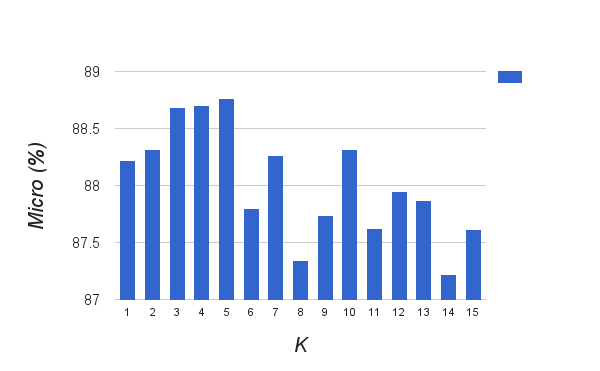
\includegraphics[width=\linewidth]{./k_effect.png}
\caption{Effect of parameter $K$ on entity linking accuracy.
Trained on CoNLL train and tested on CoNLL test-a.}
\label{fig:k_effect}
\end{figure}
}
% PGF plot version of the figure
{
\pgfplotsset{every tick label/.append style={font=\tiny}}
\begin{figure}[t!]
\centering
\resizebox {\columnwidth} {!} {
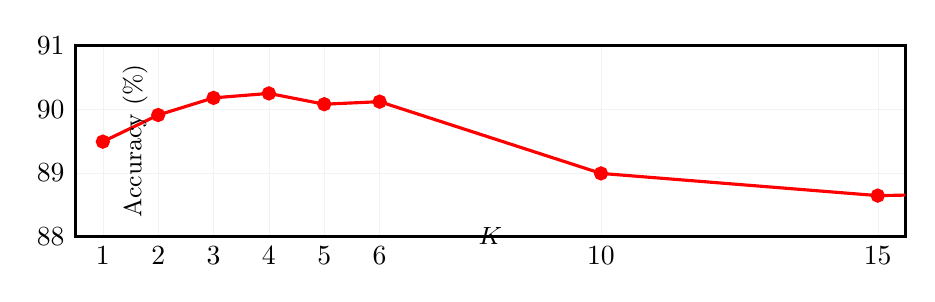
\begin{tikzpicture}
  \begin{axis}[
   %title  = Effect of K,
   width = \columnwidth,
   height=4cm,
%    ybar,
 %   bar width = 0.2cm,
    %x axis line style = { opacity = 0 },
    %axis y line       = none,
    tickwidth         = 0pt,
    xmin=0.5,xmax=15.5,
    ymin=88,ymax=91,
    grid=both,
    grid style={line width=.1pt, draw=gray!10},
    x label style={at={(axis description cs:0.5,0.1)},anchor=north},
    y label style={at={(axis description cs:0.1,.5)},anchor=south},
    xlabel={\small $K$},
    ylabel={\small Accuracy (\%)},
    mark size=2.0pt,
    line width=1.0pt,
   % enlarge y limits  = 0.2,
    xtick = data,
  ]
  \addplot [line width=0.4mm, red, mark=*, mark options=solid] coordinates { 
    (1,89.49) (2,89.91)  (3,90.18) (4,90.25) (5,90.08) (6,90.12) (10,88.99) (15,88.64) (20,88.72)
  };
  \pgfresetboundingbox
  %\addplot coordinates { (20,1)         (15,2)
   %                      (60,3)   (75,4)  };
 % \legend{Topics, Posts}
  \end{axis}
\end{tikzpicture}
}
\caption{Effect of parameter $K$ on entity linking accuracy.
Trained on CoNLL train and tested on CoNLL test-a. \label{fig:k_effect}}
\end{figure}
}

%(1,89.72) (2, 89.77) (3, 90.39) (4, 90.39) (5, 90.52)   (6,90) (7,90) (8,90) (9,90) (10,90)   (11,90) (12,90) (13,90) (14,90) (15,90)};


In \secref{sec:soft_attention} we proposed an extension of softmax smoothing to the $K$ attention case. In our experiments 
we cross-validated over a wide range of $\beta$ values, including $\beta=\infty$ which corresponds to taking
the exact sum of $K$ largest values. We found that the optimal value in most cases was large: $\beta=10, 100$, or even $\infty$. This suggests that a {\em hard} attention model, where exactly $K$ mentions are picked is adequate in the current settings.

%\subsection{Examples of gains (and losses)}



%%% Local Variables: ***
%%% mode:latex ***
%%% TeX-master: "main.tex"  ***
%%% tex-main-file: "main.tex"  ***
%%% End: ***
